\documentclass{sigplanconf}

% Email drafts to: M. George Hansen, Evan Laforge, Ketil Malde, Sonke Hahn

\usepackage{amsmath}
\usepackage{amssymb}
\usepackage{natbib}
\usepackage{multirow}
\usepackage{setspace}
\usepackage{balance}
\usepackage[all]{xy}


\include{paper}
%include paper.fmt
%format (List (a) (b)) = "[" b "]_{" a "}"
%format Result_alpha = "\Varid{Result_\alpha}"
%format *> = "\mathbin{*\hspace{-5.8px}>}"
%format **> = "\mathbin{*\!*\hspace{-5.8px}>}"
%format *>> = "\mathbin{*\hspace{-5.8px}>\!\!>}"
%format ?> = "\mathbin{\raisebox{-.7px}{?}\hspace{-4px}>}"
%format ?== = "\mathbin{\raisebox{-.7px}{?}\hspace{-4px}\equiv}"
%format `replaceExtension` = "\backtick{replaceExtension}"
%subst string a = "\!\text{\sf ``" a "\char34}\!"
%format context = "\Keyword{context}"
%format dependsS = "\Varid{depends\!^{*}}"
%format hashInclude = "\text{\sf ``\#include \textbackslash\char34\char34}"


\newcommand{\file}{\textsf}
\newcommand{\prog}{\texttt}
\newcommand{\make}{\prog{make}}

\begin{document}
\conferenceinfo{ICFP'12,} {September 10--12, 2012, Copenhagen, Denmark.}
\CopyrightYear{2012}
\copyrightdata{978-1-60558-794-3/10/09}

\preprintfooter{}   % 'preprint' option specified.

\title{Shake -- A Better Make}
% \subtitle{}

\authorinfo{Neil Mitchell}
           {\verb"ndmitchell@gmail.com"}

\maketitle

\begin{comment}
1. State the problem
2. Say why it�s an interesting problem
3. Say what your solution achieves
4. Say what follows from your solution
\end{comment}

\begin{abstract}
Build tools, such as \make{}, are typically used for compiling source code into executables. Unfortunately, most build tools fail to deal properly with generated source files, especially when the dependencies of those generated files can only be determined after the files have been generated. Generated files are common in many large software systems, resulting in awkward hacks to paper over build tool inadequacies. We describe how to generalise build tools to deal properly with generated files. We have implemented our ideas as the Haskell library Shake, which has been used by Standard Chartered for the last three years as the basis for a complex build system involving millions of lines of code in many languages.
\end{abstract}

\category{D.3}{Software}{Programming Languages}

\terms
Languages

\keywords
build-system, compilation, Haskell

\section{Introduction}
\label{sec:introduction}

A build tool, such as \make{} \cite{make}, takes a set of input files, plus some build rules, and produces some output files. Using \make{}, a build rule can be written as:

\begin{code}
{-"\textsf{result.tar : file1 file2}"-}
    {-"\textsf{tar -cf result.tar file1 file2}"-}
\end{code}

\noindent This rule says that the file \file{result.tar} depends on the inputs \file{file1} and \file{file2} (first line), and provides a command to build \file{result.tar} (second line). Whenever \file{file1} or \file{file2} change, the command will be run, and \file{result.tar} will be built.

But imagine we want to build \file{result.tar} from the list of files stored in \file{list.txt}. The dependencies of \file{result.tar} cannot be specified in advance, but depend on \textit{the contents} of \file{list.txt}. Unfortunately, \make{} offers no easy way to express this dependeny (there are workarounds, but none are pleasant or effective). Using the build tool we develop in this paper, we can write:

\begin{code}
"result.tar" *> \_ -> do
    need ["list.txt"]
    contents <- readFileLines "list.txt"
    need contents
    system' "tar" $ ["-cf","result.tar"] ++ contents
\end{code}

This rule describes how to build \file{result.tar}. We depend on (|need|) the file \file{list.txt}. We read each line from \file{list.txt} into the variable |contents| -- being a list of the files that should go into \file{result.tar}. Next, we depend on all the files in |contents|, and finally call the \prog{tar} program. If either \file{list.txt} changes, or any of the files listed by \file{list.txt} change, then \file{result.tar} will be rebuilt.

The key difference from \make{} (and nearly all other build tools) is that rather than specifying the dependencies of a rule \textit{in advance}, we allow further dependencies to be specified \textit{after} examining the results of previous dependencies. This difference is crucial to accurately describe many dependency relationships. The particular example that made us explore this is, particularly for generated files. With generated files you want to generate the file, then examine it to determine its dependencies -- the atlernative is trying to guess at it's dependencies before running the generator, which is error prone.

\todo{is this a build system for generated files? if so, argue why make doesn't do generated files. is it just about complete dependencies?}


We have implemented our build tool as a Haskell library, named Shake, which is available online\footnote{\url{http://hackage.haskell.org/package/shake}}. Shake properly handles generated files and includes the important features of \make{}, such as minimal rebuilds (running only a subset of the rules when some subset of the inputs change), and parallelising the build (running multiple independent rules at the same time). By implementing Shake as a Haskell library we allow rules to be written using the full power of Haskell, including the use of modules and functions to properly structure large build systems.

\subsection{Contributions}

\begin{itemize}
\item We describe the theory underlying \make{} (\S\ref{sec:theory_make}), and how to revise this theory to properly handle generated files (\S\ref{sec:theory_shake}).
\item We describe how to extend our theory to enable minimal rebuilds (\S\ref{sec:cached_shake}).
\item We describe how to implement our build tool in Haskell, including how to present the underlying theory in a way that is practically usable (\S\ref{sec:user_view}), and how to implement it efficiently (\S\ref{sec:developer_view}). While Haskell is not essential to implement our build tool, it offers a number of advantages -- primarily making IO effects explicit and providing nice syntactic sugar.
\item We describe how additional features can be added to our build tool, including a Lint tool (\S\ref{sec:lint}), a profiling tool (\S\ref{sec:profiling}) and a dependency analysis tool (\S\ref{sec:analysis}).
\item We allow rule dependencies and targets to be arbitrary values. While we can represent files (\S\ref{sec:file_rules}), we can also represent static configuration information, the existence of files in a directory (\S\ref{sec:exists_rule}) and commands that produce multiple results (\S\ref{sec:multiple_outputs}).
\item We have implemented a large build system using Shake (\S\ref{sec:evaluation}). The build system is 9000 of lines of Haskell, building over a million lines of source code and over a million lines of generated code, written in many programming languages. We originally implemented this build system using \make{}, but the result was slow to run, hard to maintain, and frequently caused spurious compile failures. Since using Shake, our build system has ceased to be a problem. This experience suggests a number of guidelines to follow when using Shake.
\end{itemize}


\section{Theory}
\label{sec:theory}

\todo{there should be more examples, more code, more intuition -- less detail}

In this section we describe the theory that underpins of non-recursive \make{} \cite{miller:recursive_make}, then the underlying theory of our build system, named Shake. We then describe how to support minimal rebuilds in both theories. In \S\ref{sec:user_view} and \S\ref{sec:developer_view} we show how to implement these ideas in a usable tool.

\subsection{Intuition}

Most build systems such as \make{} build a dependency graph from a set of rules, and then traverse that graph to build the result. An essential point is that the graph cannot change -- you cannot have graphs in the node which depend on things not yet defined. The fundamental problem with generated files is that you want to look at them to figure out what they depend on. The solution is to move dependency generation until after the file has been built, or other rules are built, but that means you cannot build a static graph.

Make builds a static graph, which means you can't figure out as you are going. We don't! If you just recurse from beginning to end build artifacts fall out! The key intuition is that you can specify additional dependencies, after using previous dependencies. As we saw in the previous section, additional dependencies can be specified with need.

\subsection{Theory of Make}
\label{sec:theory_make}

While the \make{} tool is heavily file based, that is not an essential property of the ideas behind \make{}. We use the type |Key| for things that can be created or are dependencies (i.e. file names) and the type |Value| for the values associated with a |Key| (i.e.  file contents). Using this abstraction, we can model \make{} as:

\begin{code}
data  Rule =
      {  creates  :: Key
      ,  depends  :: List alpha Key
      ,  action   :: List alpha Value -> Value
      }

make :: Set Rule -> Key -> Value
\end{code}

The |make| function takes a (possibly infinite) set of rules and the target |Key| to build, and returns the |Value| associated with that |Key|. A rule can be modelled as the |Key| it |creates|, the |Key|s it |depends| on, and the |action| that takes the depended upon |Value|s and produces the result |Value|. We use |List alpha bullet| to denote a list which must have length |alpha|, requiring that the |depends| list and the list passed to |action| are equal in length.

We restrict our model to only building one target, while \make{} allows multiple targets (i.e. a list of |Key|s to build). However, we can encode multiple targets by creating a distinguished rule that depends on all the targets and returns all their values, and then make that rule the single target.

\subsubsection{Correctness}

We say a |Rule| is associated with a |Key| if it has that |Key| as its |creates| field. Given a |Rule| |r| we can define |dependsS r| as all the |Key|s this rule requires to run, including the dependencies of its dependencies. We can compute |dependsS r| as the union of |depends r| and |dependsS| on all the rules associated to |depends r|.

For a call to |make| to be valid, given a set of rules and a target, we require:

\begin{enumerate}
\item \textit{No duplicate rules} - no |Key| may have two associated rules.
\item \textit{No missing rules} - every item in a |depends| list must have an associated rule.
\item \textit{Target rule} - there must be a rule associated with the target.
\item \textit{Finite} - for all rules, |dependsS r| must be finite.
\item \textit{Acyclic} - for all rules, |dependsS r| must not contain |creates r|.
\end{enumerate}

\noindent Given a valid call to |make|, there exists a finite list of |action|s that when run in order produces the result. Provided each |action| terminates, the result can be obtained.

\subsection{Theory of Shake}
\label{sec:theory_shake}

Using the same terminology from the previous section, we can model our build tool as:

\begin{code}
data  Rule =
      {  creates  :: Key
      ,  action   :: Action
      }

data Action  =  Depends Key (Value -> Action)
             |  Result Value

shake :: Set Rule -> Key -> Value
\end{code}

The |shake| function takes a (possibly infinite) set of rules and the target |Key| to build, and returns the |Value| associated with that |Key|. A rule can be modelled as the |Key| it |creates|, and the |action| that creates the result. The |Action| either returns the |Result| |Value|, or requires a new dependency with |Depends| -- specifying the |Key| it depends on, plus a function that takes the |Value| of that |Key| and provides a new |Action|.

The big difference from |make| is the introduction of dynamic dependencies. A rule can dynamically, based on the values of previous dependencies, require additional dependencies. We can easily translate a |make| |Rule| to a |shake| |Rule|, but the reverse is not true -- |shake| is strictly more powerful than |make|.

\subsubsection{Correctness}

A call to |shake| is correct if the |Value| associated with the target |Key| can be built. Unlike |make|, we cannot check this property before running any |action|s, since new dependencies can be added by running an |action|. Like |make|, we require that each |Key| is associated with exactly one |Rule|. Given a function which finds the rule associated with a key (|find|), we can run a build system as:

\begin{code}
shake rules target = fromKey target
    where
        fromKey k = fromAction (action (find rules k))

        fromAction (Result val) = val
        fromAction (Depends dep act) =
            fromAction (act (fromKey dep))
\end{code}

To reduce a |Key|, we find its |Rule| and reduce its |Action|. To reduce an |Action|, if it is a |Result| we return the value, if it is a |Depends| we reduce the dependency then reduce the result of the action. Note that in this simple implementation every time a |Key| is required we compute its |Value| from scratch -- an action may be run many times.

A call to |shake| is correct if it terminates. We can guarantee termination if:

\begin{enumerate}
\item We require that every |action| function terminates.
\item To ensure that the recursion in |fromAction| terminates, we require that |Rule| produces a finite number of |Depends| constructors before producing a |Result|.
\item To ensure that the recursion in |fromKey| terminates, we require that no |Rule| depends on its |create| value, either directly or through a sequence of other rules.
\item To ensure that the mutual recursion between |fromKey| and |fromAction| terminates, we require that there are a finite number of |Key| values required to build the |target|.
\end{enumerate}

%
% \begin{itemize}
% \item \textit{Result} rules are those whose |action| is a |Result|.
% \item \textit{Reducible} rules are those which are not \textit{results}, but where the immediate dependencies are all \textit{results}.
% \item \textit{Required} rules are those which are not \textit{results}, but which create something in the set of output keys, or who create something that a \textit{required} rule has in it's |Defer| list. We can guarantee that all \textit{required} rules must be evaluated for the build system to finish.
% \end{itemize}
%
% Like in \make{}, the rules |creates| must all be distinct.
%
% Given a set of rules, we are finished when all the \textit{required} rules are \textit{results}. We can proceed one step by taking a rule that is both \textit{required} and \textit{reducible} and running the deferred function on it (\textit{reducing} it). If there are no rules that are both \textit{required} and \textit{reducible} then we are stuck, and the build system has a logical inconsistency, either because there is no rule to build something, or the build rules form a cycle.
%
% Note that we cannot know if the build system is consistent until it has completed. In particular, there are two ways for a build system to loop. Most obviously, an \textit{required} and \textit{reducible} rule could have a deferred action that never terminates. Alternatively, such a rule could immediately produce the same dependencies as previously, without making progress. We assume that each rule is structured in a way that there are a finite number of steps, and each step takes a finite amount of time (in practice, it is hard to write a rule that does not obey this property).
%

\subsection{Minimal Rebuilds in Make}
\label{sec:cached_make}

One of the important properties of \make{} is minimal rebuilds. In any execution of |make|, each |action| will be run at most once. If the last time the action was run it had the same inputs, the action will not be repeated. The \make{} tool uses file modification times, and assumes a target is valid if all its dependencies have older modification times. We can model this behaviour with a function that looks up the modification times:

\begin{code}
history :: Key -> Maybe Value
\end{code}

If we restrict ourselves to |Key|s which are files, and |Value|s which are modification times (as \make{} does), then we can write a function |history| which returns |Just| the modification time, or |Nothing| to indicate the file does not exist (and thus has never been built). An |Rule|s |action| can be skipped if the |creates| file exists, and all the |depends| times are older. Before running a rules action, all its dependencies must already have been created, and thus history must always return |Just|. We can check if a Rule is valid with respect to the history with:

\begin{code}
validHistory :: Rule -> Bool
validHistory r = case history (creates r) of
    Nothing -> False
    Just t -> all ((< t) . fromJust . history) (depends r)
\end{code}

This scheme is limited to files, for two reasons:

\begin{enumerate}
\item Our |history| function relies on being able to access the history for a previous run which is stored on disk. We can eliminate this problem by storing the information in a database as we are executing, and then reloading it from disk on each execution.
\item Our |validHistory| function relies on a |Value| which is monotonically increasing (e.g. time). We can eliminate this problem if whenever we complete an action we give it a real timestamp.
\end{enumerate}

We can make these changes to produce:

\begin{code}
data  Info = Info
      {  value :: Value
      ,  built :: Time
      }

history :: Key -> Maybe Info

validHistory r = case history (creates r) of
    Nothing -> False
    Just i -> all ((< built i) . built . fromJust . history) (depends r)
\end{code}

However, this scheme is incorrect for |Value|s that are stored by both the file system \textit{and} in our database. Consider a file, which has a file system modification time, and also has a |Value| in our database. If the file is edited externally, then the |Value| in our database will be incorrect. We can solve this problem by also checking that, where the |Value| is stored externally, it is still consistent:

\begin{code}
data Stored = NeverStored | NotStored | Stored Value

stored :: Key -> Stored

validStored :: Key -> Value -> Bool
validStored k v = case stored k of
    NeverStored -> True
    NotStored -> False
    Stored value -> v == value
\end{code}

When attempting to read a value stored externally there are three possible states. Either the value is never stored, in which case it exists only in our database, and is always consistent. Or the value is sometimes stored, but not currently available externally -- such as a file that does not exist on disk, in which case the action must be rerun. Or the value is stored, and has an external value -- in which case the value is valid if it matches what we have stored. We can avoid running the action associated with a rule if it is valid with respect to the stored values, and with respect to the history.

In order to remain consistent throughout the execution, we require that all |stored| values do \textit{not} change during the execution, other than as a result of running an |action| which |creates| it. The \make{} tool requires a similar property or it becomes inconsistent.

While the timestamp approach works reasonably for \make{}, it can fail if the system clock changes, or if a file is modified but has its value set to an older timestamp -- such as when extracting a backup which resets the timestamp. Instead of relying on the system time, we can instead store a counter in our database, and increment it every time we require a time value, thus guaranteeing that our time is correctly ordered.

After running an action, we typically store a new time in the |history|. However, if the result of the |action| has not changed we \textit{do not} update the time. This allows any files that depend on this file to avoid recalculation, which can significantly reduce the number of actions that need to be run.

\subsection{Minimal Rebuilds in Shake}
\label{sec:cached_shake}

Our original algorithm calculated every file repeatedly. We can easily add a cache mapping |Key| to |Value| and avoid reducing a rule that has already been reduced in this execution.

To obtain minimal rebuilds across executions we can use the same approach as described in the previous section. However, we cannot determine whether a |history| is valid based on the rule, as we do not have the |depends| available, and do not want to rerun the |action| just to get the dependencies. Therefore, we just store the dependencies alongside.

\begin{code}
data  Info = Info
      {  value :: Value
      ,  built :: Time
      ,  depends :: [Key]
      }

history :: Key -> Maybe Info

validHistory r = case history (creates r) of
    Nothing -> False
    Just i ->
        all ((< built i) . built . fromJust . history) (depends i)
\end{code}

\noindent We can reuse the |validStored| unmodified.

\subsubsection{Unchanging Files}
\label{sec:unchanging_files}

Now let us consider the case where a rule runs, but the result is the same as last time. As an example, consider a generated source file. If the generator changes it is necessary to regenerate the file, but there is a chance the result will be the same. In \make{}, the solution is to disallow such changes, and always \prog{touch} the result after a rule completes. However, we can do better, avoiding unnecessary computation.

Instead of storing just the built time, we can also store the |changed| time. Whenever we build a file we update its |built| time, but if the value is the same as last time, we leave its |changed| time the same. When checking |validHistory| we can replace the condition as:

\begin{code}
all ((< built i) . changed . fromJust . history) (dependsUpon i)
\end{code}

By introducing two timestamps for a single |Key|, we can reduce the number of builds required. For certain practical examples, this improvement can reduce rebuild times after a change from many minutes to seconds.

\section{Shake in Haskell}
\label{sec:user_view}

In order to make the theory from \S\ref{sec:theory} practically usable as a Haskell library, we need to make a number of design decisions. In particular, we describe how to replace |Key| and |Value| with standard polymorphic values, how to integrate IO into the |action| function and how to define an infinite set of rules. We first present the interface to Shake, then in \S\ref{sec:developer_view} we describe how to implement the internals of the library.

\subsection{A Shake Example}

\begin{figure}
\begin{code}
import Development.Shake
import System.FilePath

main = shake def $ do
    want ["Main"]

    "Main" *> exe -> do
        cs <- getDirectoryFiles "." "*.c"
        let os = map (`replaceExtension` "o") cs
        need os
        system' "gcc" $ ["-o",exe] ++ os

    "*.o" *> \o -> do
        let c = replaceExtension o "c"
        need [c]
        headers <- liftIO (cIncludes c)
        need headers
        system' "gcc" ["-o",o,"-c",c]
\end{code}
\caption{Demo build system in Shake.}
\label{fig:demo}
\end{figure}

We give an example Shake program in Figure \ref{fig:demo}. Running this program will build \file{Main} from all the \file{*.c} files in the current directory. If we add or remove a \file{.c} file, or change any of the \file{.c} files or the header files they @#include@, then the necessary files will be recompiled.

The script produces (|want|'s) the file \file{Main}. To generate \file{Main} we list all the \file{*.c} files in the current directory, change their extensions to \file{*.o}, require those files to be built (|need| them), then call \prog{gcc} to link them. To build any \file{*.o} file we take the associated \file{*.c}, make sure it's been built, then call the function |cIncludes| to get all headers it includes (|cIncludes| can be defined in terms of \prog{gcc -M}). We require those headers, then we call \prog{gcc} to do the compilation.

This script demonstrates a number of features of Shake based build systems:

\begin{itemize}
\item It's a full Haskell program with a |main| entry point. While |main| can simply call |shake|, it can also do anything it likes, such as command line processing (see \S\ref{sec:command_line}).
\item The call to |getDirectoryFiles| is tracked (see \S\ref{sec:other_rule_types}), if the results change, it will trigger a rebuild.
\item We run arbitrary system commands in the internals.
\item We fully track the dynamic dependencies introduced by header files. The function |cIncludes| given a source file returns all the files required by transitive @#include@ directives. (In \S\ref{sec:transitive} we show a better way to define transitive dependencies.)
\end{itemize}

\subsection{Core Shake}

\begin{figure}
\begin{code}
data  ShakeOptions = ShakeOptions
      {  shakeFiles :: FilePath
      ,  shakeParallel :: Int
      ,  ellipses
      }
    deriving (Default)

data Rules a
    deriving (Monad, Monoid)

data Action a
    deriving (Monad, LiftIO)

class (
    Show key, Show value,
    Typeable key, Typeable value,
    Hashable key, Hashable value,
    Eq key, Eq value,
    Binary key, Binary value,
    NFData key, NFData value
    ) => Rule key value | key -> value where
    validStored :: key -> value -> IO Bool
    validStored k v = return True

run :: ShakeOptions -> Rules () -> IO ()

action :: Make a -> Rules ()

rule, defaultRule :: Rule key value =>
    (key -> Maybe (Make value)) -> Rules ()

apply :: Rule key value => List alpha key -> Make (List alpha value)
apply1 :: Rule key value => key -> Make value
\end{code}
\caption{Primitive operations in Shake}
\label{fig:shake_core}
\end{figure}

The primitive interface to Shake is given in Figure \ref{fig:shake_core} -- everything else is defined on top. At its essence, a Shake build system is a set of rules. We can run the rules with |run|, create new rules with |rule|/|defaultRule|/|action|, and when defining a rule we can express a dependency with |apply|/|apply1|.

We execute a set of rules with the |run| function, which also takes an options record. Typical options include which file to store the cached versions in (|shakeFiles|), and the number of processors to use (|shakeParallel|). These options are also used to select which mode to run Shake in, as described in \S\ref{sec:tools}.

Every rule that is defined or applied in Shake must be a member of the |Rule| class. The |Rule| class defines the method |validStored| to determine whether a value is consistent with the value stored externally. We require that each rule |key| has only one type of |value|, this restriction is not technically required, but forces users to keep their rules simple. Each |key|/|value| type must also be in several type classes:

\begin{description}
\item [Typeable] We allow multiple types of rules in a single build system. To distinguish the types, and to match on only one type at a time, we require a |Typeable| constraint, allowing us to obtain an explicit |TypeRep| \cite{lammel:syb}.
\item [Eq] We require equality to match the values.
\item [Binary] We require |Binary| so we can store the values in a database, to achieve minimal rebuilds.
\item [Hashable] We require |Hashable| to perform fast searching.
\item [Show] We require |Show| for debugging messages and logging.
\item [NFData] We require |NFData| to ensure that values are fully evaluated when they are computed, ensuring that errors happen at the appropriate place.
\end{description}

Standard Shake rules are defined with |rule|, which requires a function which takes a single |key| value, and returns |Nothing| to indicate that this rule does not build this |key|, or |Just| with the steps necessary to build the associated |value|. If two rules match the same key then an error is raised. The function |defaultRule| allows a rule to be defined with a lower priority, which is used if no standard rules match -- for an example see \S\ref{sec:file_rules}. Instead of defining targets to build, we allow rules with no target, which are always run. The |Rules| type is a |Monoid|, allowing two sets of rules to be appended to produce a new set of |Rules|. In practice, the syntactic sugar supported by |Monad| is often a more natural way to define rules in a build system, so we also make |Rules| a |Monad|. The |Action| type is a |Monad| and has an instance for |MonadIO|, allowing users to call arbitrary |IO| functions using |liftIO| to translate |IO alpha| to |Action alpha|.

The |apply1| function takes a |key|, builds it, and returns the associated |value|. The |apply1| function finds a rule of the appropriate type whose application returns |Just|, then runs the action. The |apply| function can be thought of as |mapM apply1|, but is defined to build all necessary dependencies in parallel (see \S\ref{sec:parallelism}).

We have deliberately kept the core of Shake small and extensible, supporting all instantiations of |Key|/|Value| outside, thus focusing purely on the building side. We describe how to implement this core in \S\ref{sec:developer_view}.

\subsection{Defining Rule Types}
\label{sec:exists_rule}

To work correctly, the |key|/|value| types of |apply1| and |rule| must match each other. To aid end users, we suggest that most rule authors define sugar functions, as we have done for the rule types included with Shake. The simplest rule available is one that determines if a file exists, similar to the standard function |System.Directory.doesFileExist|, but where the dependency is tracked. As an example, consider the following rule:

\begin{code}
".config" *> \dest -> do
    b <- doesFileExist ".config.user"
    let src = if b then ".config.user" else ".config.default"
    copyFile src dest
\end{code}

This rule creates \file{.config} by copying either \file{.config.user} if it exists, or otherwise copying \file{.config.default}. The intention is that there is a default configuration, but it can be overridden by then user. Note the use of dynamic dependencies -- if the user has a \file{.config.user}, and the \file{.config.default} changes then the rule will not be run, however if the file didn't exist it would be.

\begin{figure}
\begin{code}
import System.Directory as IO

newtype Exist = Exist FilePath
    deriving (Typeable, Show, Eq, Hashable, Binary, NFData)

instance Rule Exist Bool where
    validStored (Exist x) b = liftM (== b) $ IO.doesFileExist x

doesFileExist :: FilePath -> Action Bool
doesFileExist = apply1 . Exist

defaultRuleDoesFileExist :: Rules ()
defaultRuleDoesFileExist =
    defaultRule $ \(Exist x) -> Just $
        liftIO $ IO.doesFileExist x
\end{code}
\caption{Implementation of |doesFileExist|.}
\label{fig:doesfileexist}
\end{figure}

We define |doesFileExist| in Figure \ref{fig:doesfileexist}. We first define a |newtype| wrapper to represent the |key| type, deriving all the necessary classes. We define an instance for |Rule Exist Bool|, where |validStored| simply checks that the existence of the file matches. We define |doesFileExist| as very gentle sugar around |apply1|, the primary purpose is to tie down the types, so users cannot make mistakes. Finally we define a |defaultRule| which runs the action. Anyone wishing to use |doesFileExist| should include |defaultRuleDoesFileExist| in their rule set.

We use a restricted module export list to export only |doesFileExist| and |defaultRuleDoesFileExist|, and thus we are guaranteed that the types match. Note that if a value changes we are likely to call |IO.doesFileExist| twice in a row, once to invalidate the old value in |validStored|, and once to compute the new value in |default_|. We can alleviate this problem with a single element cache -- although in practice we find it not to be a problem, since the operating system typically caches all file queries.

We end with a note of caution. We require that any stored value remains consistent other than when a rule actively changes in. Since this rule does not force the existence of a file, it should not be used on any files that may be generated by the build system -- |doesFileExist| should return the same at the start and end of the compilation. This property can be checked with Lint mode as described in \S\ref{sec:lint}.

\subsection{File Based Rules}
\label{sec:file_rules}

\begin{figure}
\begin{code}
import System.Directory as IO

newtype File = File FilePath
newtype FileTime = FileTime Int
-- plus all necessary instances

getFileTime :: FilePath -> IO (Maybe FileTime)
getFileTime x = do
    b <- IO.doesFileExist x
    if not b then return Nothing else do
        TOD t _ <- IO.getModificationTime x
        return $ Just $ FileTime $ fromIntegral t

instance Rule File FileTime where
    validStored (File x) t = fmap (== Just t) $ getFileTime x

need :: [FilePath] -> Action ()
need xs = (apply $ map File xs :: Action [FileTime]) >> return ()

defaultRuleFile :: Rules ()
defaultRuleFile = defaultRule $ \(File x) -> Just $ do
    res <- liftIO $ getFileTime x
    let msg = "Error, file does not exist and no rule: " ++ x
    return $ fromMaybe (error msg) res

want :: [FilePath] -> Rules ()
want xs = action $ need xs

(?>) :: (FilePath -> Bool) -> (FilePath -> Action ()) -> Rules ()
(?>) test act = rule $ \(File x) ->
    if not $ test x then Nothing else Just $ do
        liftIO $ createDirectoryIfMissing True $ takeDirectory x
        act x
        res <- liftIO $ getFileTime x
        let msg = "Error, rule failed to build the file: " ++ x
        return $ fromMaybe (error msg) res

(**>) :: [FilePattern] -> (FilePath -> Action ()) -> Rules ()
(**>) test act = (\x -> any (x ?==) test) ?> act

(*>) :: FilePattern -> (FilePath -> Action ()) -> Rules ()
(*>) test act = (test ?==) ?> act
\end{code}
\caption{Implement of file rules.}
\label{fig:file_rules}
\end{figure}

While our build system is not restricted to rules dealing with files, in practice many build systems are file orientated. For files, the filename is a sensible |Key|, but |Value| could be either the on-disk modification time or a hash of the file contents (e.g. SHA1). We found in that modification time is faster (significantly faster for large files) and being able to rebuild something with \prog{touch} is highly convenient! Of course, our design allows anyone to define a new file type, based on file hashes. Using modification time for values, we define the functions for working with files in Figure \ref{fig:file_rules}.

To force files to be built, we define |need| and |want|. The |need| action demands all the modification times associated with the filenames, then throws away the result -- a computation depends on the time a file was built, but rarely uses the modification time in its computation. We define |want| as simply a |need| run as an action.

We define |defaultRuleFile| as a rule that simply checks if the file is already present, and if so uses it. Source files will have no associated rules, so this rule just records their modification time. If a file has no rules (since any rules would be run in preference to the default rule), and does not exist, then we give an error to the user. As with |defaultRuleDoesFileExist|, anyone using |want|/|need| should include |defaultRuleFile| in their rule set.

We define new file rules with |(?>)|, which takes a predicate to match against the file name and an action to run. This function forces the correct types, and obtains the modification time afterwards. Before running the action we create the directory containing the output file, an idea taken from the Ninja build system \cite{ninja}. We found that when running a large set of newly written rules, often one rule would create the output directory while another did not -- meaning some rule orderings worked while others failed. Automatically creating the output directory removes this source of failure.

While |(?>)| is the ultimate file creation rule, we define two additional operators, in terms of a wildcard match operator |(?==)|. We define |(*>)| for matching a single pattern, for example |"*.c" *> ellipses|, in a very similar manner to \make{}. We also define |(**>)| for matching any one of a set of patterns. In our large evaluation, we found that |(?>)| was used about 5\% of the time, |(**>)| was used about 10\% and |(*>)| was used about 85\% of the time. In our experience, use of |(?>)| is a sign that the build system is poorly designed and should be rethought (our large evaluation used |(?>)| exclusively for compatibility with the system it replaced).

As a practical concern, when writing file rules, often there are multiple types of object that build \file{*.o} files. This problem can be easily solved by making Haskell produce \file{*.hs.o}, C produce \file{*.c.o} etc.


\subsection{Automatically Include Default Rules}
\label{sec:include_default_rules}
\label{sec:other_rule_types}

With the rule types already defined, users can write a build system using Shake. Unfortunately, if the user forgets to include the rule |defaultRuleFile|, there is likely to be a runtime error. Instead of requiring the user to remember to include the default rules, we instead define a wrapper function |shake| which includes all default rules available:

\begin{code}
shake opts rules = run opts $ do
    defaultRuleDoesFileExist
    defaultRuleFile
    ellipses
    rules
\end{code}

The astute reader may be wondering why we can't move |defaultRule| into the |Rule| type class, and avoid requiring such a wrapper. Alas, that solution doesn't work for reasons described in \S\ref{sec:dynamically_typed}, because we always need to have an explicit rules of each type to deserialise dynamically typed values.

We also include a bunch of other rules, including a tracked version of |getDirectoryFiles|, oracle information etc. \todo{complete this}

\subsection{Additional Functions}
\label{sec:derived}

Using the file rules from the previous section, we can define new versions of operations such as |readFile|/|copyFile|, which automatically call |need|:

\begin{code}
readFile' :: FilePath -> Action String
readFile' x = need [x] >> liftIO (readFile x)

copyFile' :: FilePath -> FilePath -> Action ()
copyFile' old new = need [old] >> liftIO (copyFile old new)
\end{code}

These operations mirror their standard counterparts, but automatically include a |need| call. It is never harmful to include an additional call to |need|, in fact, sometimes it is beneficial! Consider the following example:

\begin{code}
"file.txt" *> \out -> do
    need [out ++ ".part1", out ++ ".part2"]
    part1 <- readFile' (out ++ ".part1")
    part2 <- readFile' (out ++ ".part2")
    writeFile' out (part1++part2)
\end{code}

Here we use the additional function |writeFile'|, simply |writeFile| lifted to the |Action| monad. This rule would work correctly without the |need| call on the second line, as both |readFile'| calls include |need| within them. However, when running the build system in parallel, the additional |need| allows both dependencies to be computed at the same time, while the |need| calls inside |readFile'| serialise building of the dependencies.

We define a number of additional functions for working with files. The functions |readFileLines|/|writeFileLines| deal with files which should be treated as a list of lines. The function |writeFileChanged| writes a file, but only if the contents have changed, and is useful for avoiding redundant computation due to unchanging files (see \S\ref{sec:unchanging_files}).

We define the |system'| function which take a list of command line arguments, and escapes them as necessary, before calling the underlying |system| command. This function also contributes generates profiling information (see \S\ref{sec:profiling}). The |system'| function should be used carefully, as it cannot tell which files the system command may depend on, so explicit |need| commands must be used (see \S\ref{sec:lint} for ways to detect such a problem). We recommend writing wrappers around system commands which insert the appropriate |need| calls.


\section{Implementing Shake}
\label{sec:developer_view}

We have implemented Shake, and used it extensively. In this section we sketch some of the central implementation challenges, and how they can be overcome. Readers interested in the full implementation are welcome to download the associated package (see \S\ref{sec:introduction} for a link). In the implementation of Shake there are several goals:

\begin{description}
\item[Correctness] -- we always execute enough rules to obtain correctness, but we never rebuild something that could be reused.
\item[Efficiency] -- we aim to make the implementation efficient, while remembering that often executing a rule is expensive.
\item[Parallelism] -- we try and do lots of work in parallel where possible.
\item[Error feedback] -- if the build system fails for some reason, such as the rules being incorrect as per \S\ref{sec:theory_shake}, then it's nice to give useful error messages. While this may sometimes conflict with efficiency (maintaining extra state to only be used in an error), it is necessary to make Shake usable.
\end{description}

\subsection{Dynamically Typed Values}
\label{sec:dynamically_typed}

A single Shake program can use multiple types of keys and values. To work with heterogenous values in Haskell we define:

\ignore\begin{code}
data Any = Any (forall alpha bullet
    (  Typeable alpha, Eq alpha, Binary alpha
    ,  Hashable alpha, Show alpha, NFData alpha) => alpha)
\end{code}

This definition, using existentials \cite{laufer:existentials}, allows anything supporting all the type classes required to be stored with type |Any|. We can define |Key| and |Value| types in terms of |Any|. We can implement |Eq|, |Show|, |Hashable| and |NFData| instances for |Any| without difficulty, often by appealing to the |TypeRep| provided by the |Typeable| instance.

Implementing a |Binary| instance for |Any| is harder. Serialising a value is easy, but deserialising a value is problematic -- we can deserialise a |TypeRep|, but then we need to obtain the |get| method from the |Binary| instance associated with that type. The solution is to keep a table mapping |TypeRep|s to |Any| values containing the appropriate |Binary| instance. This table must include every type stored in the file we are reading, or it cannot be deserialised. We populate the table using all rules defined by |rule| and |defaultRule| in |Rules| -- which means we cannot move |defaultRule| into the |Rule| type class, as then a type could be usefully used without appearing in |Rules|, and would not be missing from the table.

When deserialising, if we encounter a type not present in the table, we ignore the entire database. This is pessimistic, but safe -- if the set of types has changed that implies the build system has changed, which is not tracked anyway (see \S\ref{sec:changing_rules}).

\subsection{Shake State}
\label{sec:parallelism}

\begin{figure}
\begin{code}
type State = Map Key Status

data Status  =  Loaded Info
             |  Building (MVar ()) (Maybe Info)
             |  Built Info

data  Info = Info
      {  value :: Value
      ,  built :: Time
      ,  changed :: Time
      ,  depends :: [[Key]]
      }
\end{code}

\xymatrix{
 & \mathsf{Loaded}\ar@@/_1pc/[dr]^{Invalid}\ar@@/^1pc/[rr]^{Valid} & & \mathsf{Built} \\
\mathsf{Database}\ar@@{-->}[ur] & & \mathsf{Building}\ar@@/_1pc/[ur]^{Finished} \\
& \mathsf{Missing}\ar@@{-->}[ur]
}
\caption{The state of a Shake process.}
\label{fig:state}
\end{figure}

\todo{is this really the right state to track? figure out how to build stuff}

The state of a running Shake program can be represented by the data type in Figure \ref{fig:state}. The |State| is a mapping from |Key| to |Status|, giving the status of each key the build system knows about. The |Status| data type has three constructors:

\begin{description}
\item[|Loaded|] is used for information that has been loaded from the database, but not yet checked against its history, or any stored value it may have.
\item[|Building|] is used for a rule that is currently running, or has been queued for execution. If a key is needed that is already building, the thread that requires it should wait on the |MVar| until that rule has completed.
\item[|Built|] is used for rules that were loaded and valid, or have finished building.
\end{description}

The |Status| constructors also take an |Info|, which contains the same fields as in \S\ref{sec:unchanging_files}, with one modification. To allow full parallelism when rebuilding dependent rules, we store |depends| as |[[Key]]| instead of just |[Key]| -- where each entry comes from one call to |apply|. When saving |State| to the database, we ignore the |Status| fields and save only the |Key|/|Info| mapping.

With this state, it is relatively easy to implement the core of Shake -- the functions which are actually responsible for building account for less than 100 lines, most of which is dealing with parallelism. We execute the top-level |actions|, and whenever we call |apply|, we look up the state in the database, and use the transition diagram in Figure \ref{fig:state} to make sure everything is |Built| before continuing.

To implement parallelism we use the \prog{parallel-io} \cite{parallel-io} library to queue up rules to be run, which ensures we never have more than a user specified number of rules executing in parallel. The \prog{parallel-io} library deliberately randomises the order of computations it runs, as a result of the needs of Shake. By randomising the rules, we provoke failures earlier than we would other have. In addition, some stages of a build require different resources -- for example the compiler requires CPU while the linker requires disk access. If we are not careful, we can result in executing all compilers followed by all linkers. Using random ordering means we get a better mix, which gives a noticeable speedup -- measured at 20\% for some practical workloads.

When running a large build system, it is common for it to fail before completing -- either because a rule raised an error, or the end user killing the build process. In these cases it is important that none of the work that has been performed is lost -- therefore we maintain a journal and every time a rule transitions from |Building| to |Built| we write that information immediately. If Shake completes successfully we delete the journal. If on restarting Shake has a journal file, we replay the journal onto the database.

You have to be non-deterministic! If you find someone is changed, you can kick off a build immediately. However, if you find they are dirty, you want to give up. Whichever gets checked first will end up winning, but the alternative is waiting until you know, which is a bad plan.

You may run entirely redundant rules, since once you start, you finish. A good idea for resource management.

\subsection{Error Messages}

To improve error messages we make a number of changes from the natural implementation:

\begin{itemize}
\item We maintain a stack for each executing rule, containing the rules that required it. Whenever we invoke a rule, we check the stack for recursion in rules, giving a clear error message where otherwise there would have been an infinite loop.
\item Whenever an error occurs, either when running a rule or trying to find a rule, we print the stack. The stack is particularly useful when there is no rule for a file, but the fact that file is required is itself suspicious.
\item We have options to print every rule run, and every system command run. Whenever a system command fails, we reprint the command line after the failure.
\end{itemize}

\section{Evaluation}
\label{sec:evaluation}

We have used a build system based on Shake at Standard Chartered for the last three years. Our build system has been an unqualified success -- while the complexity of our project has increased (more files in more languages with more preprocessors), the build system is no more complex. When we introduced Shake it replaced an extensive \make{} based system, which contained over 10,000 lines of make files, was regularly incorrect and very slow. Switching to Shake made our build system 10 times shorter and halved build times. In a single run our build system typically checks 360,000 rules.

% Our build system has a maximum of 20 levels deep of |apply| calls from the top-level |action| statement, but 80\% of build rules are between 3 and 7 steps deep.

% [(0,2127),(1,22651),(2,190623),(3,64795),(4,15666),(5,22732),(6,10583),(7,11801),(8,5658),(9,5035),(10,3144),(11,2500),(12,974),(13,605),(14,251),(15,230),(16,73),(17,25),(18,25),(19,6),(20,1)]

In implementing our build system we have learnt a number of lessons -- both about best practices for structuring build systems, and how the underlying core of Shake can be used to deal with the complexities of real development. In this section we share some of those lessons.

\subsection{Command Line Interface}
\label{sec:command_line}

While the |shake| function can be used as |main|, it offers no support for command line arguments. We use the |shake| function to build a program \prog{mk}, which handles command line options, allowing us to specify some of the fields in |ShakeOptions| (Figure \ref{fig:shake_core}), such as parallelism and verbosity.

One essential feature of any build tool is the @clean@ command, which deletes all build objects. Using Shake we could query the database to find all build results, and delete them. Alternatively, deleting the database will cause a full rebuild. However, we have found the most convenient solution is to create all build objects in a folder \file{.make}, and clean our project by deleting that directory.

Using \make{}, you can specify build targets on the command line. We provide an enhanced version of this feature, allowing both individual files and sets of files to be enabled/disabled. As an example, a user may write @mk !DOCS@ to disable building documentation, or @mk index.html@ to build only \file{index.html}. We control these targets by passing a modified version of |want| to the functions specifying rules, which consults the command line arguments:

\begin{code}
documentation :: (String -> [FilePath] -> Rules()) -> Rules ()
documentation wants = do
    wants "DOCS" ["index.html"]
    "index.html" *> \out -> ellipses
\end{code}

\subsection{Multiple Outputs}
\label{sec:multiple_outputs}

Some programs, such as the Haskell compiler \prog{ghc} \cite{ghc7_2}, can produce two outputs from one action -- compiling \file{Foo.hs} produces both \file{Foo.o} and \file{Foo.hi}. As a first approximation, the \file{.o} file depends on the entire contents of the file, while the \file{.hi} file depends only on the type signatures. A single \prog{ghc} invocation needs to do all the work to produce both, but often the \file{.hi} file will be left unchanged. Unfortunately, many build systems (including \make{}) do not handle multiple outputs well.

In Shake, it is usually possible to fake multiple outputs with single file dependencies -- claiming that \file{Foo.hi} depends on \file{Foo.o} with no action and \file{Foo.o} depends on \file{Foo.hs} by running \prog{ghc}. Thanks to support for unchanging files (see \S\ref{sec:unchanging_files}), the \file{.hi} file will not cause a rebuild unless it changes. However, this rule has two problems:

\begin{itemize}
\item If \file{Foo.hi} is deleted \textit{without} also deleting \file{Foo.o}, then \file{Foo.hi} will not be rebuilt and the build system will be incorrect.
\item If \prog{ghc} updates \file{Foo.hi}, but manages to determine it does not need to update \file{Foo.o}, then \file{Foo.hi} will not be marked as dirty and the build will be incorrect.
\end{itemize}

Despite these limitations, the fake single file dependency is usually sufficient. However, consider a command that reads \file{numbers.txt} containing lines of numbers, and produces \file{even.txt} and \file{odd.txt} -- each containing only the even or odd numbers -- but does not update an output file that has not changed. In this situation there is no fake dependency that properly captures the flow of updates. Fortunately, we can capture the proper meaning by introducing a new type or rule, for rules which produce multiple files.

\begin{code}
data Files = Files [FilePath]
data FileTimes = FileTimes [Int]

multipleOutputs = do
    rule $ \(Files xs) ->
        if xs /= ["even.txt","odd.txt"] then Nothing else Just $ do
            need ["numbers.txt"]
            system' "number-split" []
            liftM FileTimes $ mapM getFileTime xs

    ["even.txt","odd.txt"] **> \_ ->
        apply1 $ Files ["even.txt","odd.txt"]
\end{code}

Inside |multipleOutputs|, the call to |rule| declares a rule that can build both \file{even.txt} and \file{odd.txt} in a single step. We call the \prog{number-split} program, and get the file times for the results. On the |**>| line we define two rules to produce the output files, using the standard file creation rules as in Figure \ref{fig:file_rules}, by calling |apply1| with the list of files to create. If the build first requires \file{even.txt} then \prog{number-split} will be invoked, but a subsequent requirement on \file{odd.txt} will not force the program to be rerun.

The Shake library provides a function |*>>| to capture this pattern, allowing an end user to write:

\begin{code}
["even.txt","odd.txt"] *>> \_ ->
    need ["numbers.txt"]
    system' "number-split" []
\end{code}

\subsection{Transitive Dependencies}
\label{sec:transitive}

In build systems, it is common for the system to require the transitive dependencies. As an example, if \file{foo.c} does a @#include@ on \file{bar.h}, and \file{bar.h} in turn includes \file{baz.h}, then \file{foo.c} should be recompiled if either \file{bar.h} \textit{or} \file{baz.h} changes. A similar situation arises when linking Haskell programs -- any module transitively imported by the root module should be linked in. One option is to separately for each \file{*.c} file, scan all its dependencies and |need| them. However, that can significantly reduce performance, as if \file{bar.h} is included hundreds of times then it will be recomputed lots. We can also define a more specific one, based on the assumption that @#ifdef@ statements do not change the include files (a reasonable assumption in many cases).

Therefore, a standard pattern is to define \file{*.dep} as the immediate dependencies of a file, and \file{*.deps} as the transitive dependencies. Returning to the C include file example:

\begin{code}
"*.deps" *> \out -> do
    dep <- readFileLines $ replaceExtension out "dep"
    deps <- mapM (readFileLines . (<.> "deps")) dep
    writeFileLines out $ nub $ dep ++ concat deps

["*.c.dep","*.h.dep"] **> \out -> do
    src <- readFileLines $ dropExtension out
    let incs = [init y  |  x <- src
                        ,  Just y <- [stripPrefix hashInclude x]]
    writeFileLines out incs

"*.c.o" *> \out -> do
    need =<< readFileLines (replaceExtension out "deps")
    system' "gcc" ["-c",dropExtension out,"-o",out]
\end{code}

\subsection{Build rules that change}
\label{sec:changing_rules}

Throughout this work, we assume that \textit{the build system does not change}, merely the inputs to the build system. While the build system does change more rarely than the rest of the code, in our case about 1.7\% of commits have touched the build system. However, there have been only a handful of times when a build system change required a complete rebuild to be performed. We manage build system changes with a number of strategies:

\paragraph{A \textsf{shakeVersion} field in \textsf{ShakeOptions}} We have a field named |shakeVersion| in the |ShakeOptions| record defined in Figure \ref{fig:shake_core}. If the build system changes in a significant and incompatible way, then this flag can be incremented to force a full rebuild. This is the nuclear option -- we have only had 8 such occurrences in the last three years, and none recently (as we have learnt how Shake can be used best).

\paragraph{Depending on the build source file} A conservative strategy is to depend on the build system in each rule, and then if any of the build system changes rebuild everything from scratch. While that is an option, it would cause a significant number of redundant rebuilds. Instead, where we have files that specify code generators, which could conceptually be stored in separate programs, we put an explicit dependency and use |writeFileChanged| (see \S\ref{sec:derived}). Now, if the generator changes it will be run again, but typically only a handful of files will see an actual change, so very little is rebuilt.

\paragraph{Make the build system interpret} Much information, such as what files a \file{*.c} file includes, can be computed from the source files. Where information cannot be computed, such as which files should be linked together to form an executable, we write small rule files which list the inputs to an object. The standard rule for linking depends on these rule files, and thus if the rules about what goes into an executable change the file is automatically rebuilt.

\paragraph{Restarting rules} If Shake detects that a dependency has changed, it rebuilds the rule from the beginning. Due to the presence of the |[[Key]]| |depends| field, it never checks for rules that the previous step did not permit. The result is that most changes cause something in the dependencies to change, and thus the rule is rerun anyway.

\smallskip\smallskip

In practice we have not found changing the build system to be problematic. By moving settings out of the build system, into separate tracked rule files, and using the |shakeVersion| flag as a last resort, we see no issues. However, the only correct way to deal with a changing build system would be functional equality -- something that would be particularly useful to Shake.

\section{User Tools}
\label{sec:tools}

In addition to standard build functionality, Shake also provides additional features to make build tool authors lives easier. In this section we describe three features that have been built on top of Shake -- a profiling tool to determine what took most time, an analysis tool to query the build dependencies and a lint tool to check that the build system is sensible.

\subsection{Profiling}
\label{sec:profiling}

Shake records two separate pieces of profiling information.

\paragraph{Rule execution times} When running a rule we record the execution time, excluding any time to build its dependencies. From this information, we can determine which rules are most expensive. This information can be aggregated from different build runs, allowing us to produce a total build time, ignoring parallelism, even if only a handful of rules were executed in the last run.

\paragraph{Traced IO actions} Most time consuming rules invoke IO actions, typically system commands. We provide a trace function:

\begin{code}
traced :: String -> IO alpha -> Action alpha
\end{code}

\noindent All actions run by |traced| are stored by the rule that invoked them, along with a human readable message (the first argument), and the start and end times. We automatically call |traced| when running system commands. The execution time of IO actions can be aggregated from different build runs, similar to rule execution times. In addition, taking only IO actions from a single run, we can determine how many IO actions were executing at each point in time -- allowing us to produce a parallelism graph as shown in Figure \ref{fig:profile}.

\smallskip\smallskip

We have built profiling support into the core of Shake. Since any execution of a rule is likely to take some time (most rules will be spawning system processes), the overhead of profiling information is negligible. In previous versions of Shake we only recorded profiling information when explicitly asked, but found that users often wanted to profile the build run that had just completed -- always recording profile information makes that possible.

\subsection{Analysis}
\label{sec:analysis}

The Shake database records the dependencies of each item, allowing a full dependency graph to be produced after the rules have been run. However, for any project of moderate size, a picture of the dependency graph is rarely comprehensible -- although through judicious filtering it is possible to produce something useful (see Figure \ref{fig:analysis} for an example). Instead, we have found value in that writing passes to answer specific questions, such as:

\begin{itemize}
\item Why was a particular file rebuilt in the last build run? Shake shows the complete path of dependencies.
\item If I touch a file, what will rebuild? Shake computes the list of rules that depend on that file, including indirect dependencies, but assuming no unchanging files (see \S\ref{sec:unchanging_files}.
\item What is the most expensive file to change? For each leaf of the graph, Shake computes all dependencies, and then uses execution times from profiling to determine the most expensive file.
\item Do my dependencies follow some layering principle? For example, I would not expect any files outside |Development.Shake.*| to import any modules from inside that module tree, other than |Development.Shake| itself. Many large projects are structured into isolated layers, which can be validated by the build system.
\end{itemize}

Shake can export the full dependency graph, so additional queries can be written.

There have been alternative attempts at visualising build systems, such as \cite{adams:maintaining_build_systems}, which could be applied to the full dependency graph, and can scale much better.

\subsection{Profiling and Analysis}

\begin{figure}
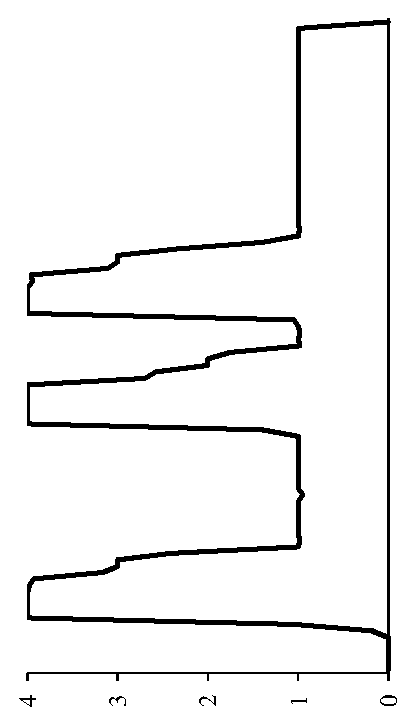
\includegraphics[scale=0.7,angle=270]{profile.eps}
\caption{Build parallelism.}
\label{fig:profile}
\end{figure}

\begin{figure}
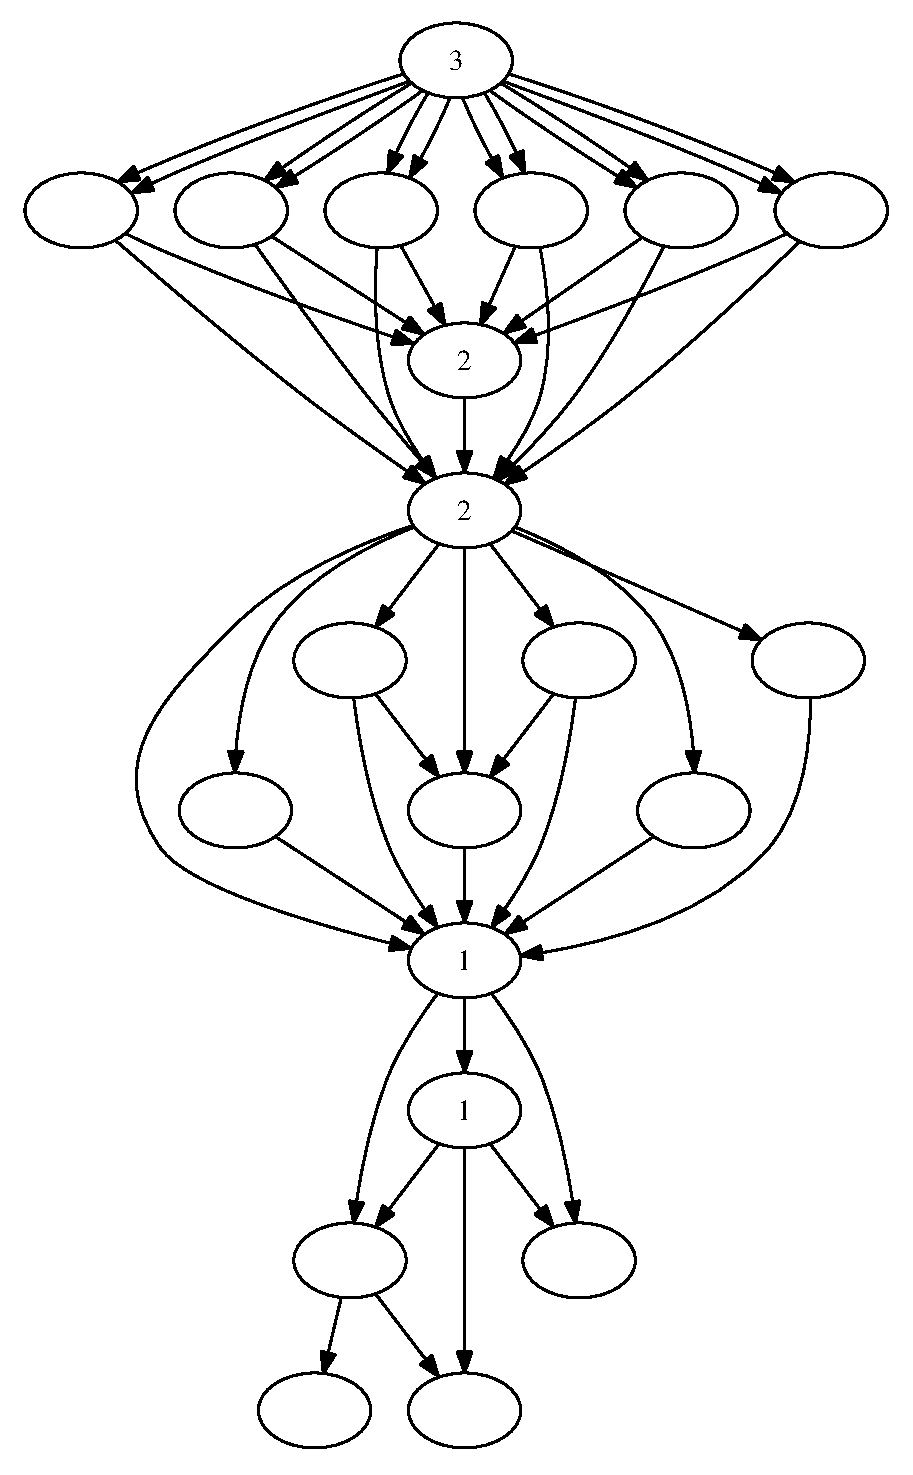
\includegraphics[scale=0.5]{layout.eps}
\caption{Dependency graph.}
\label{fig:analysis}
\end{figure}

% REVISED NUMBERS on a laptop:
% GHC build = 7.141 full, 0.453 minimal
% Shake build = 11.828 full, 0.101 minimal (of which 0.6 is ghc-pkg, 75% of the rest is writing the db)
% When making, make sure you turn off profiling output, to get better benchmark numbers

As an example of the profiling and analysis tools in practice, see Figures \ref{fig:profile} and \ref{fig:analysis}. Both these diagrams are produced by building a 24 module Haskell program\footnote{The program is Shake itself, which can be compiled using Shake.} from scratch with a maximum of four processors. The entire process takes 6.35 seconds, but spends 11.82 seconds executing rules, giving a parallel speed up of 1.9 times. Executing the build system with no parallelism takes 11.57 seconds (likely due to reduced disk contention). \todo{confirm on desktop}

Figure \ref{fig:profile} shows the number of traced system commands executing at any point during the build. We see a start up period where zero commands are running and the build system is checking for dependencies, followed by three spikes up to four processors, followed by a tail of using one processor.

Turning to the dependency graph in Figure \ref{fig:analysis}, we have the |Main| module at the top labelled 3. This graph shows the dependencies of the \file{.hi} files, after hiding three leaf utility modules which are include in many places and have no dependencies (they add lots of lines, obscuring the real dependency graph). It is clear the build proceeds in three stages, with bottle-neck dependencies marked 1, 2 and 3. These three dependencies account for the three periods of one processor usage. The final tail of one processor includes both compilation of the main module (which profiling tells us takes 0.23 seconds) and linking (which takes 2.31 seconds).

This example shows how Shake's profiling and analysis reports can be used to improve build performance. If the bottle-neck modules could be split up, or if their compilation time was reduced (particularly for those marked 1, which account for a longer single processor section), the overall build speed would increase. In practice, we have found that for large build systems, where Shake is building multiple targets, the parallelism usually stays at the maximum (or fractionally below it) for most of the build time, before reducing down to one processor as the last few tasks complete.

\subsubsection{Comparison to @ghc --make@}

Building the same project with the GHC compilation system \cite{ghc7_2}, using \prog{ghc --make}, takes 10.70 seconds, compared to Shake with 11.57 seconds for one processor and 6.35 seconds for four processors. The reason GHC is quicker on one processor is that GHC keeps all interface information and package database information in memory, whereas running separate \prog{ghc -c} compilation commands requires reloading this information each time. However, Shake is able to use parallelism to improve the build time, while GHC cannot.

% if we compile with -O1 instead of -O0 then GHC=13.375 while Shake=18.375, so it gets worse for Shake

When running the build system while nothing needs compiling, GHC takes 0.54 seconds and Shake takes 0.12 seconds. Of the 0.12 seconds required by Shake, 0.9 seconds is spent checking the GHC installation has not changed (running @ghc --version@ and @ghc-pkg list@) -- if the GHC installation is assumed to be constant Shake requires only 0.03 seconds. Shake is faster because it reads in one file (the database) then quickly checks |validStored| on a small number of files. GHC must at least query the same file information, but also has to construct a dependency graph, aggregating information from many files.

% Compared to something like gcc, which is always invoked in single mode, we do better.
% For something like C# we don't have a choice and always run it in --make mode.

\subsection{Lint checking}
\label{sec:lint}

\todo{write lint checking}

Writing a large build system is a complex endeavour.

Can we roll it right back? Look which files a system command uses, and from that build the profiling report? Might work better on Windows.


There are two primary things we check for with lint. To get a full build we build everything, run whatever clean action the user has specified, then rerun each rule. The best lint will come if you:

* clean everything, apart from the database
* build with --lint

It's important when rebuilding to require the rules bottom up, i.e. the want statements should be replaced with something doing a bottom up traversal.

lint with invariants can always be done very easily.

lint with observations is much harder, since you don't want observations to overlap. that means you have to run the rules bottom up. or can try and subtract rules?

\subsubsection{Invariant information}

Things like whether a file exists or not should be constant throughout, otherwise any files which don't know will get confused. This can be checked by cleaning, and then running. Any key that marks itself as invariant should not change during this process. To do so, we add to the |Rule| class:

\begin{code}
invariant :: key -> Bool
invariant _ = False
\end{code}

\subsubsection{Dependency creation}

When running a file we can ask what has been changed, and what has been used. When we run just a rule, but no dependencies, the list of things that change must all be things who had rules run on them, and the list of things that were used should be equivalent.

\begin{code}
data Observed alpha = Observed {created :: Maybe [alpha], used :: Maybe [alpha]}

observed :: IO alpha -> IO (Observed key, alpha)
observed act = do res <- act; return (Observed Nothing Nothing, res)
\end{code}

Note that our original design simply passed an |IO ()| to observed, and required the function to execute it. Alas, this went wrong since it's too easy to write an incorrect version that fails to execute! Now, thanks to parametricity, if you don't pass an error back, you must have got it right!

Given a set of observations, we can check what a key used in its body, and what it declared to create. However, there are a number of situations where people don't write 100\% accurate dependencies, but the effect is equivalent. For example, assuming \file{temporary.txt} is unused in the result of the build system, the following two rules seem morally equivalent:

\begin{code}
"foo.txt" *> \out -> copyFile "bar.txt" out

"foo.txt" *> \_ -> need ["temporary.txt"]
"temporary.txt" *> \out -> do
    copyFile "bar.txt" "foo.txt"
    writeFileLines "temporary.txt" []
\end{code}

We can imagine more complex examples, and do define such examples in \ref{sec:multiple_outputs}. Therefore, we require the following properties:

\begin{itemize}
\item If you create a key that someone else requires, you must be a dependency of them.
\item If you use a key, you must depend on that key directly.
\item If you use a key but do not require it, you are safe, but conservative.
\end{itemize}

\section{Related Work}
\label{sec:related_work}

\todo{references}
\todo{cite recursive make considered harmful}

Build systems can be divided into two categories -- those which target single-language projects with fixed rules (e.g. \prog{ocamlbuild}, \prog{ghc --make}, Visual Studio projects), and those which are more general allowing user specified rules (e.g. \make{} and Shake). Focusing on the second category, the defacto standard is \make{}, but there are many \make{} competitors (notably Ant, CMake, Jam, Scons and Waf). Most of these tools read a rule list, generate a dependency graph, then execute commands while traversing that graph.

Since the number of build systems is vast, we have focused on four build systems which take different approaches (Redo, Ninja, Fabricate and Tup). Interestingly, the main thing all four systems have in common is that they require some external database of build data, in addition to the rules and file system. Unlike Shake, all these build systems are strictly limited to files.

\subsection{Redo}

% https://github.com/apenwarr/redo

The Redo build system \cite{redo} is certainly the most similar to Shake in its underlying theory. Rules are run starting at the target. A rule may call |redo-ifchange| (similar to |need|) to ensure that this rule is repeated if any of the file arguments change. Rules can be specified to build either a specific named file, or a set of files ending with a particular extension -- more precise rules can be implemented by defining a single rule with different behaviors based on the output filename.

While Redo is similar to Shake in theory, the practical implementation is significantly different, resulting in different levels of power. Instead of having a single rule store, Redo stores each rule in a separate file, and the script language is simply shell script, where |redo-ifchange| is a program. The advantage of separate files is that Redo is able to depend on the actual rule to build the output, meaning if the build system changes the correct and minimal build elements will be rebuilt. However, separating each build rule makes it harder to reason about the build system, and eliminates many potential uses of abstraction \cite{jonge:build_components}. Redo does not support unchanging files, doesn't work on Windows, and has no support for multiple outputs.

\subsection{Ninja}

% http://martine.github.com/ninja/manual.html

The Ninja build system \cite{ninja} is designed as a two-stage build system -- users specify their build rules in some high-level manner, which is then translated to a set of Ninja build rules. As a result, the Ninja build system is not designed to be general purpose and configuration choices are expected to be resolved by the first level. The Ninja target language supports three dependency features beyond \make{}. Firstly, a rule can depend on the list of files contained in another file, allowing dynamic dependencies. Secondly, the command line for each rule is tracked, resulting in a rebuild if the rule itself changes. Thirdly, a rule can generate multiple outputs, which are properly tracked.

\subsection{Tup}

% http://gittup.org/tup/build_system_rules_and_algorithms.pdf

The Tup build system \cite{tup} is designed as an incremental build system. Tup has a similar dependency structure to \make{}, but has a significantly different implementation. Instead of scanning all dependencies, it expects the operating system to supply a list of changed files, avoiding the overhead of checking which files have changed. For large build systems the result can be a significant speed improvement for builds with few files to rebuild. We believe a similar implementation strategy could be applied to Shake, also turning it into an incremental system.

Another significant difference in Tup is the automatic treatment of dead build objects. If a rule to build \file{foo} is deleted from the rule list, then Tup automatically deletes the file \file{foo}. The problem of old build objects can be serious, resulting in builds succeeding that should have failed, and that will fail as soon as a clean build is performed (to alleviate this risk, we use an overnight build which starts from scratch). However, we have a configuration which generates a basic IDE project file, which is then modified by the user -- deleting that file after the build rule disappears would be most unwelcome. We could add support for deleting dead build objects to Shake, but chose not to.

\subsection{Fabricate}

% http://code.google.com/p/fabricate/

The key innovation in the Fabricate build system \cite{fabricate} is that dependencies do not need to be given explicitly. A build system is described as a Python program, which primarily executes system commands in order. While executing the commands, Fabricate uses system tracing (strace on Linux) to record which files are accessed. In future runs, if the same system command is reached but none of its required files have changed, the command is skipped. The resulting build systems are simple, and avoid the difficulties of correctly specifying dependencies.

There are two inherent difficulties for designing a build system without explicit dependencies. Firstly, the system tracing mechanisms on different platforms are varied, and in particular on Windows are somewhat fragile, requiring hooking system libraries or checking for last-access times. Secondly, parallelism needs to be expressed manually -- Fabricate requires the addition of explicit grouping annotations before parallelism can be used.

\subsection{Haskell Build Libraries}

There are a surprising number of Haskell libraries implementing a full dependency based build system -- we are aware of ten excluding Shake (Abba, Blueprint, Coadjute, Cake, Cake\footnote{There are two distinct build libraries for Haskell named Cake!}, Hake, Hmk, Nemesis, OpenShake and Zoom). Of these, the two Cake libraries and OpenShake are derived from an early presentation of the principles behind Shake, before the source code was available. The primary difference from the Cake libraries is that Shake as presented in this paper allows multiple different types of build rule, while the Cake libraries only allow file rules. Compared to OpenShake \cite{openshake}, we have opted to have |rule|/|apply| based on dynamic types, and then expect everyone to use sugared versions to regain static guarantees of type safety. In contrast, OpenShake uses type functions \cite{schrijvers:type_functions} to statically track the available rule types, reducing the complexity of serialisation (see \S\ref{sec:dynamically_typed}), but increasing the complexity of the library -- but compared to the similarities, this difference is minor.

\section{Conclusions}
\label{sec:conclusions}

\todo{write conclusion}

We have shown how build systems can be generalised to support generated files.

Shake is awesome. Any future work goes here.

We present Shake, a new build system based on a more powerful approach, which can do things \make{} cannot -- including handling generated files properly. We have implemented Shake in Haskell, as a Haskell library, and it is used heavily -- compiling 10's of millions of lines of code per day.

Surveys have found that about 15\% of development work is expended on the build system \cite{mcintosh:build_maintenance}, we do far less.

Build systems are an essential part of any large software project.

Implement the lint system.

\subsection*{Acknowledgements}

Thanks to Standard Chartered, where the software was developed. Thanks to Raphael Montelatici for the name Shake. Thanks to Max Bolingbroke and Evan Laforge for many discussions about Shake.


\bibliographystyle{plainnat}
\balance
\bibliography

\end{document}
